\documentclass[14pt, a4paper]{extarticle}

\usepackage[utf8]{inputenc}
\usepackage[T1]{fontenc}
\usepackage{amsmath}
\usepackage{amssymb}
\usepackage{graphicx}
\usepackage[left=2.00cm, right=2.00cm, top=2.00cm, bottom=2.00cm]{geometry}
\usepackage[russian]{babel}

\usepackage{setspace}
\usepackage{fancyhdr}

\graphicspath{{img/}}

\RequirePackage{caption}
\captionsetup[figure]{justification=centering,name=Рисунок,labelsep=endash}

\usepackage{indentfirst}

\usepackage{float}

\usepackage{titlesec}
\titleformat{\section}{\normalfont\bfseries}{\thesection~}{0em}{}

\begin{document}
	\onehalfspacing
	\begin{titlepage}
	\begin{center}
		\begin{small}
			\textbf{Министерство науки и высшего образования Российской Федерации}

			ФЕДЕРАЛЬНОЕ ГОСУДАРСТВЕННОЕ АВТОНОМНОЕ ОБРАЗОВАТЕЛЬНОЕ УЧРЕЖДЕНИЕ ВЫСШЕГО ОБРАЗОВАНИЯ
			
			\textbf{<<НАЦИОНАЛЬНЫЙ ИССЛЕДОВАТЕЛЬСКИЙ УНИВЕРСИТЕТ ИТМО>>}
		\end{small}
		
		\vspace{8em}
		
		Отчет по лабораторной работе №4
		
		РОБАСТНОЕ УПРАВЛЕНИЕ ЛИНЕЙНЫМ МНОГОМЕРНЫМ ОБЪЕКТОМ ПО СОСТОЯНИЮ
		
		По дисциплине <<Адаптивное и робастное управление>>
	\end{center}
	
	\vspace{8em}
	
	\begin{flushright}
		Выполнил:\\
		студент группы R42331c\\
		Манахов~С.П.
		
		\vspace{1em}
		
		Преподаватель:\\
		Парамонов~А.В.
	\end{flushright}

	\vfill
	
	\begin{center}
		\small
		Санкт-Петербург\\
		2022 г.\\
	\end{center}
\end{titlepage}
	\setcounter{page}{2}
	
	\section*{Задание}
	
	Дан асимптотически устойчивый объект управления:
	$$\begin{cases}
		\dot{x} = Ax + bu, x(0),\\
		y = Cx,
	\end{cases}$$
	где $x$ -- недоступный прямому измерению вектор состояния, $u, y$ -- входной и выходной сигналы объекта, доступные прямым измерениям,
	$$\begin{matrix}
		A=\left[\begin{matrix}
			-a_{n-1} & 1 & \cdots & 0 \\
			-a_{n-1} & 0 & \cdots & 0 \\
			\vdots & \vdots & \ddots & 1 \\
			-a_0 & 0 & \cdots & 0 \\
		\end{matrix}\right], & b=\left[\begin{matrix}
			0 \\ \vdots \\ 0 \\ b_m \\ \vdots \\ b_0 \\
		\end{matrix}\right], & C=\left[\begin{matrix}
			1 & 0 & \cdots & 0
		\end{matrix}\right],
	\end{matrix}$$
	$a_i,i=\overline{0,n-1},b_j,j=\overline{0,m}$ -- неизвестные коэффициенты модели.
	
	Рассматриваемая задача состоит в построении оценки вектора состояния $\hat{x}$ такой, что:
	$$\lim\limits_{t\to\infty}\left|\left|x(t)-\hat{x}(t)\right|\right|=0$$
	
	Синтезируемый адаптивный наблюдатель должен одновременно оценивать неизвестные параметры объекта управления $\theta$ и генерировать оценку вектора состояния $\hat{x}$.

	\begin{enumerate}
		\item На основе результатов, полученных в работе~№5, промоделировать адаптивный наблюдатель вектора состояния объекта. Коэффициент адаптации $\gamma$ выбрать экспериментальным путем. Построить два графика моделирования. На первом отобразить норму разности: $$\left|\left|x-\hat{x}\right|\right|=\sqrt{(x-\hat{x})^T(x-\hat{x})}$$ На втором графике -- параметрические ошибки $\tilde{\theta}$;
		\item Повторить эксперимент при $u=10sint+5cos2t+4cos4t+3cos8t$;
		\item По результатам моделирования сделать выводы.
 	\end{enumerate}
	\begin{table}[H]
		\centering
		\begin{tabular}{|c|c|c|c|c|c|c|c|}
			\hline
			Вариант & $a_1$ & $a_0$ & $b_1$ & $b_0$ & $k_1$ & $k_0$ & Сигнал \\\hline
			18 & 3 & 4 & 3 & 6 & $2\sqrt{2}$ & 4 & $u = sint+0,5cos2t$ \\\hline
		\end{tabular}
	\end{table}
	
	\newpage
	
	\section*{Описание работы}
	
	\begin{enumerate}
		\item Полученная модель состоит из настраиваемой модели:
		$$\hat{y}=\hat{\theta}^T\omega,$$
		алгоритма адаптации:
		$$\dot{\hat{\theta}}=\gamma\omega\varepsilon$$
		и алгоритма оценивания вектора состояния:
		$$\hat{x}=\sum_{i=0}^{n-1}\hat{\theta}_{i+1}\left(sI-A_0\right)^{-1} e_{n-1}\left[y\right] + \sum_{j=0}^{m}\hat{\theta}_{j+1+n}\left(sI-A_0\right)^{-1} e_{m-j}\left[u\right]$$
		
		Построенная в пакете \textit{Simulink} модель системы представлена на рисунках \ref{fig:1-system}, \ref{fig:1-properties}.
		
		\begin{figure}[H]
			\centering
			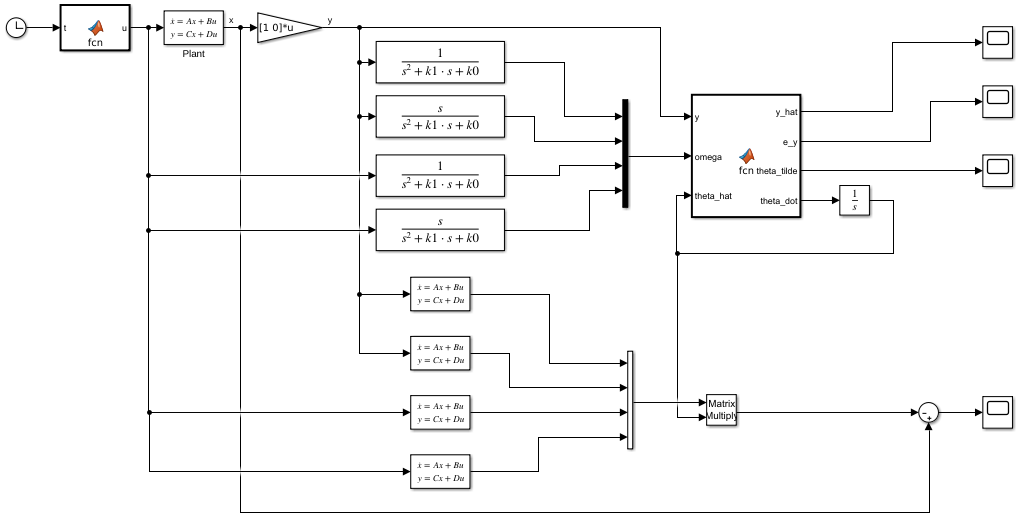
\includegraphics[width=1\textwidth]{1-system}
			\caption{Система с адаптивным наблюдателем}
			\label{fig:1-system}
		\end{figure}
		
		\begin{figure}[H]
			\centering
			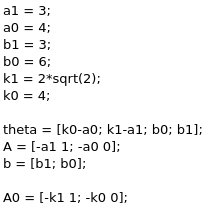
\includegraphics{1-properties}
			\caption{Параметры системы}
			\label{fig:1-properties}
		\end{figure}
		
		Полученные графики при управляющем сигнале $u=sint+0,5cos2t$ представлены на рисунках \ref{fig:1-x}, \ref{fig:1-theta}.
		
		\begin{figure}[H]
			\centering
			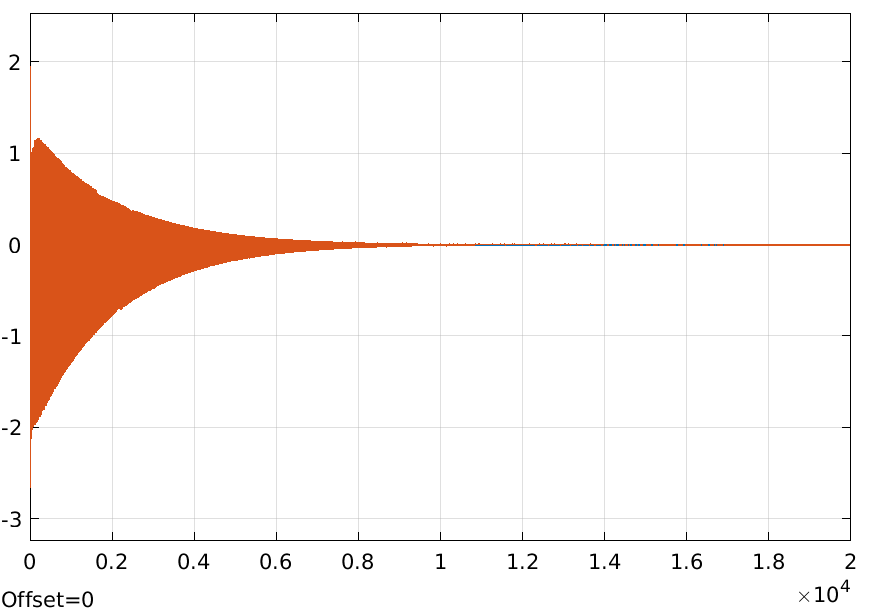
\includegraphics[width=0.59\textwidth]{1-x}
			\caption{Ошибка наблюдения вектора состояния $\left|\left|x-\hat{x}\right|\right|$}
			\label{fig:1-x}
		\end{figure}
		
		\begin{figure}[H]
			\centering
			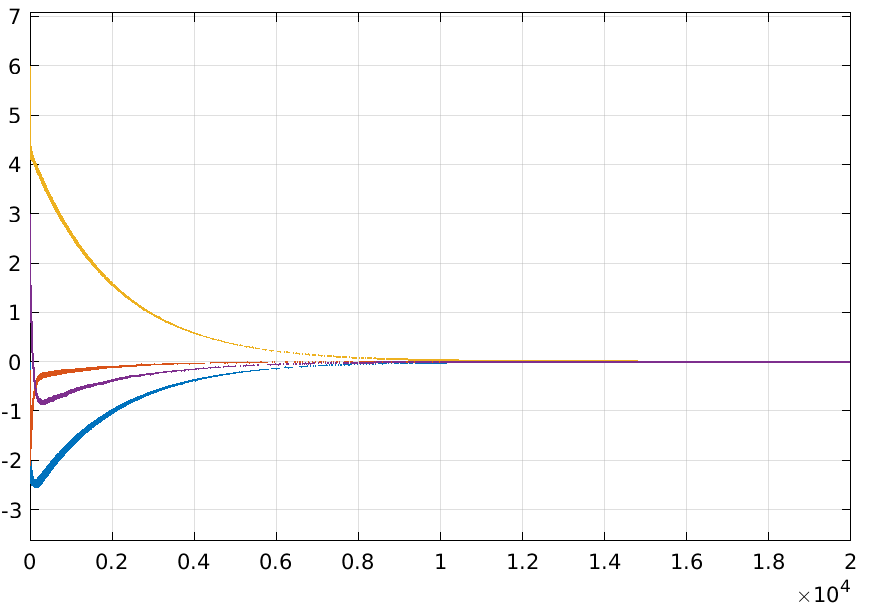
\includegraphics[width=0.59\textwidth]{1-theta}
			\caption{Параметрические ошибки $\tilde{\theta}$}
			\label{fig:1-theta}
		\end{figure}
		
		\item Полученные графики при управляющем сигнале $u=10sint+5cos2t + 4cos4t+3cos8t$ представлены на рисунках \ref{fig:2-x}, \ref{fig:2-theta}.
		
		\begin{figure}[H]
			\centering
			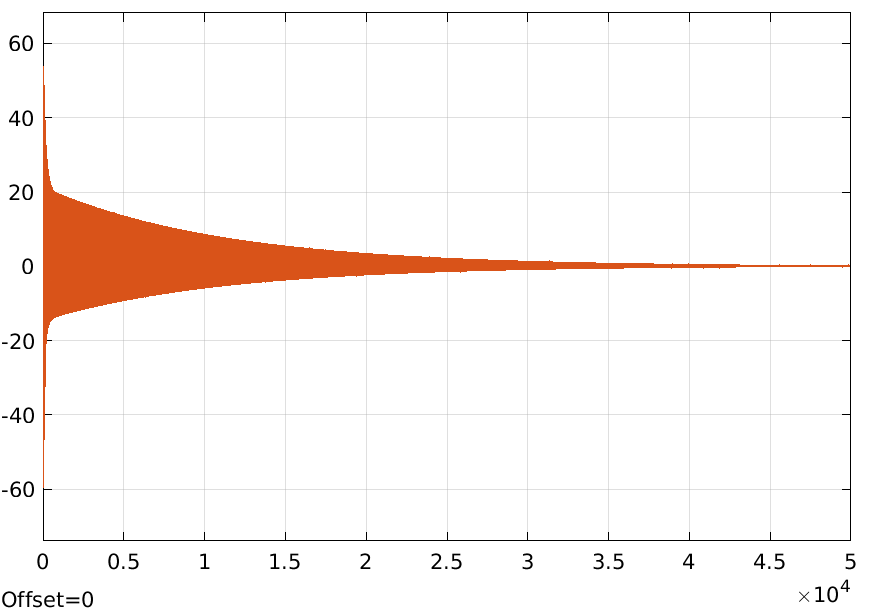
\includegraphics[width=0.59\textwidth]{2-x}
			\caption{Ошибка наблюдения вектора состояния $\left|\left|x-\hat{x}\right|\right|$}
			\label{fig:2-x}
		\end{figure}
		
		\begin{figure}[H]
			\centering
			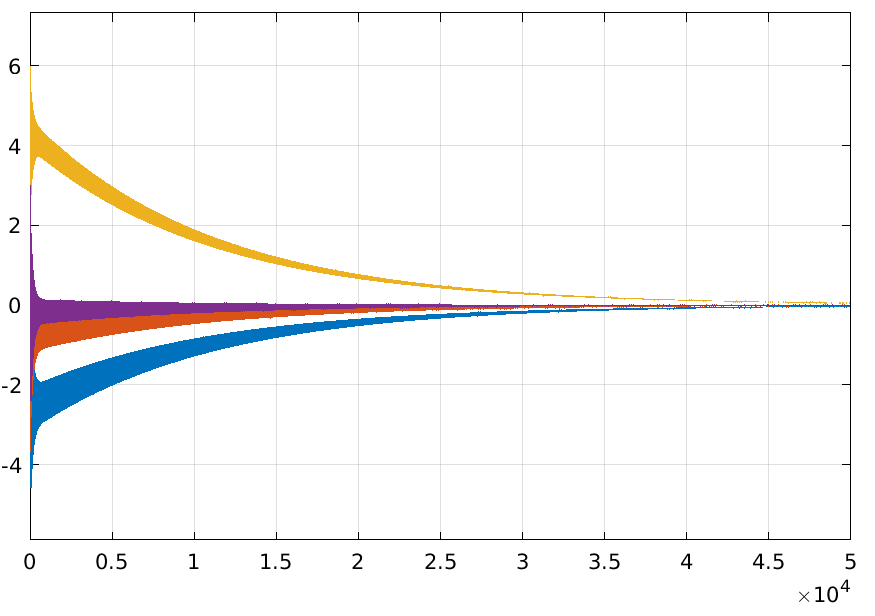
\includegraphics[width=0.59\textwidth]{2-theta}
			\caption{Параметрические ошибки $\tilde{\theta}$}
			\label{fig:2-theta}
		\end{figure}
		
	\end{enumerate}
	
	\newpage
	
	\section*{Вывод}
	
	Полученный адаптивный наблюдатель обеспечивает выполнение целевого условия при выполнении условия неисчезающего возбуждения. Проблемой является большое время оценивания.
	
	Также при увеличении числа гармоник управляющего сигнала время оценивания резко возрастает.
	
\end{document}